%%%%%%%%%%%%%%%%%%%%%%%%%%%%%%%%%%%%%%%%%
% Beamer Presentation
% LaTeX Template
% Version 1.0 (10/11/12)
%
% This template has been downloaded from:
% http://www.LaTeXTemplates.com
%
% License:
% CC BY-NC-SA 3.0 (http://creativecommons.org/licenses/by-nc-sa/3.0/)
%
%%%%%%%%%%%%%%%%%%%%%%%%%%%%%%%%%%%%%%%%%

%----------------------------------------------------------------------------------------
%	PACKAGES AND THEMES
%----------------------------------------------------------------------------------------

\documentclass{beamer}

\mode<presentation> {

% The Beamer class comes with a number of default slide themes
% which change the colors and layouts of slides. Below this is a list
% of all the themes, uncomment each in turn to see what they look like.

%\usetheme{default}
%\usetheme{AnnArbor}
%\usetheme{Antibes}
%\usetheme{Bergen}
%\usetheme{Berkeley}
%\usetheme{Berlin}
%\usetheme{Boadilla}
%\usetheme{CambridgeUS}
%\usetheme{Copenhagen}
%\usetheme{Darmstadt}
%\usetheme{Dresden}
%\usetheme{Frankfurt}
%\usetheme{Goettingen}
%\usetheme{Hannover}
%\usetheme{Ilmenau}
%\usetheme{JuanLesPins}
%\usetheme{Luebeck}
\usetheme{Madrid}
%\usetheme{Malmoe}
%\usetheme{Marburg}
%\usetheme{Montpellier}
%\usetheme{PaloAlto}
%\usetheme{Pittsburgh}
%\usetheme{Rochester}
%\usetheme{Singapore}
%\usetheme{Szeged}
%\usetheme{Warsaw}

% As well as themes, the Beamer class has a number of color themes
% for any slide theme. Uncomment each of these in turn to see how it
% changes the colors of your current slide theme.

%\usecolortheme{albatross}
%\usecolortheme{beaver}
%\usecolortheme{beetle}
%\usecolortheme{crane}
%\usecolortheme{dolphin}
%\usecolortheme{dove}
%\usecolortheme{fly}
%\usecolortheme{lily}
%\usecolortheme{orchid}
%\usecolortheme{rose}
%\usecolortheme{seagull}
%\usecolortheme{seahorse}
%\usecolortheme{whale}
%\usecolortheme{wolverine}

%\setbeamertemplate{footline} % To remove the footer line in all slides uncomment this line
%\setbeamertemplate{footline}[page number] % To replace the footer line in all slides with a simple slide count uncomment this line

%\setbeamertemplate{navigation symbols}{} % To remove the navigation symbols from the bottom of all slides uncomment this line
}

\usepackage{graphicx} % Allows including images
\usepackage{booktabs} % Allows the use of \toprule, \midrule and \bottomrule in tables
\usepackage{hyperref}
\usepackage{tikz}
\usepackage{amsmath}

%----------------------------------------------------------------------------------------
%	TITLE PAGE
%----------------------------------------------------------------------------------------

\title[Systems and control theory]{Systems and control theory} % The short title appears at the bottom of every slide, the full title is only on the title page

\author{} % Your name
\institute[KU Leuven] % Your institution as it will appear on the bottom of every slide, may be shorthand to save space
{
Katholieke Universiteit Leuven \\ % Your institution for the title page
\medskip
\textit{} % Your email address
}
\date{\today} % Date, can be changed to a custom date

\begin{document}

\begin{frame}
\titlepage % Print the title page as the first slide
\end{frame}

\begin{frame}
\frametitle{Overview} % Table of contents slide, comment this block out to remove it
\tableofcontents % Throughout your presentation, if you choose to use \section{} and \subsection{} commands, these will automatically be printed on this slide as an overview of your presentation
\end{frame}

%----------------------------------------------------------------------------------------
%	PRESENTATION SLIDES
%----------------------------------------------------------------------------------------

\begin{frame}
\frametitle{Dynamical system}
A dynamical system is a constantly changing system that connects outputs (denoted by \textbf y) and inputs (denoted by \textbf u).\\The word dynamical refers to the fact that the system relates time-changing signals.
\begin{figure}
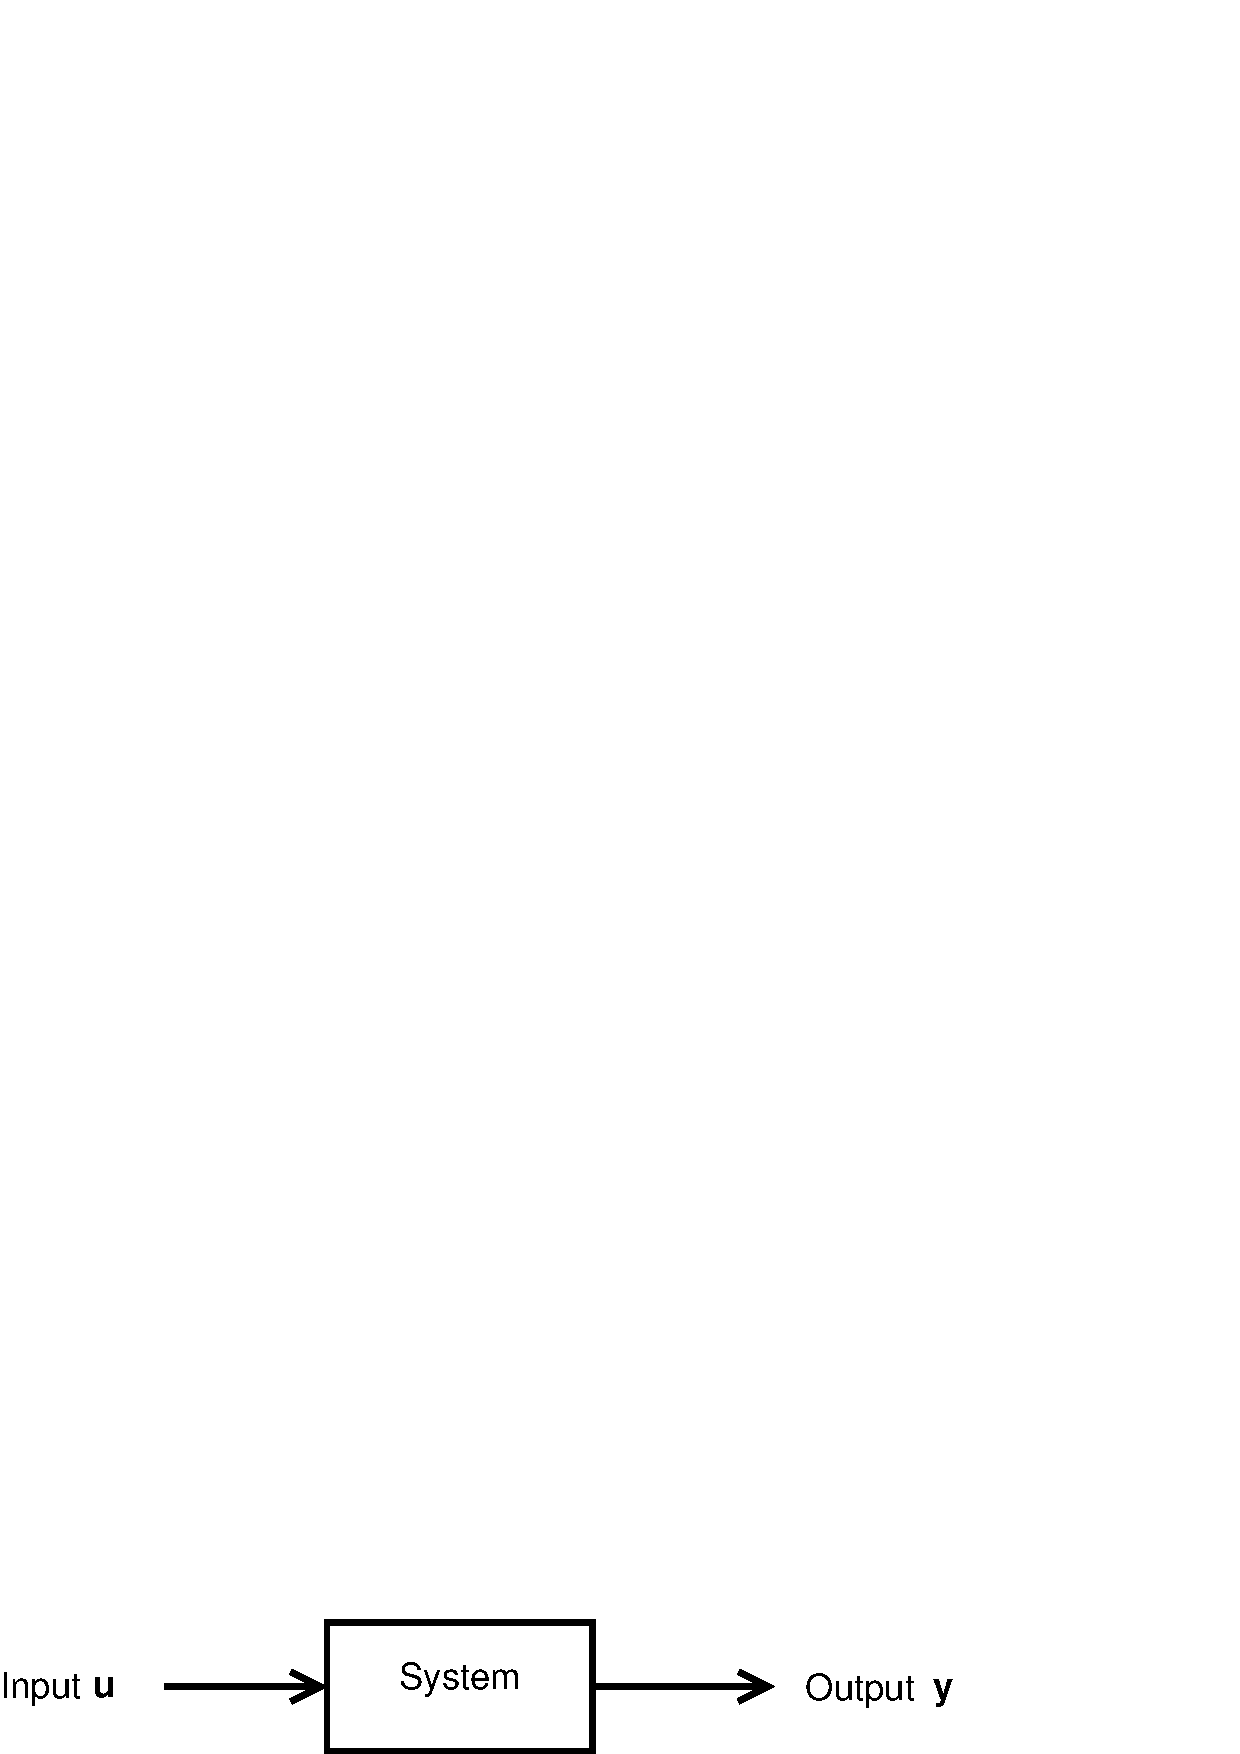
\includegraphics[width=0.8\linewidth]{Dynamical_system}
\end{figure}
\medskip
Everything is a dynamical system.
\end{frame}

%------------------------------------------------

\begin{frame}
\frametitle{Everything is a dynamical system}
\textbf{Antique racecar}
\begin{figure}
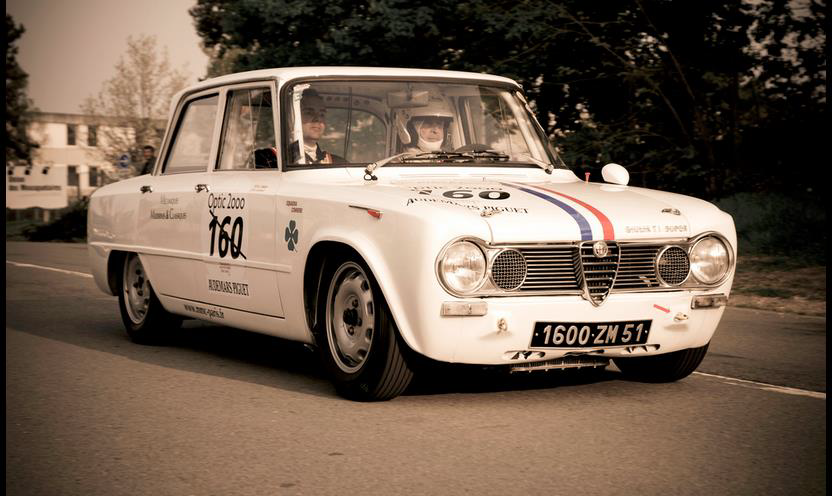
\includegraphics[width=0.9\linewidth]{racecar}
\end{figure}
\end{frame}

%------------------------------------------------

\begin{frame}
\frametitle{Everything is a dynamical system}
\textbf{Predator-prey system}
\begin{figure}
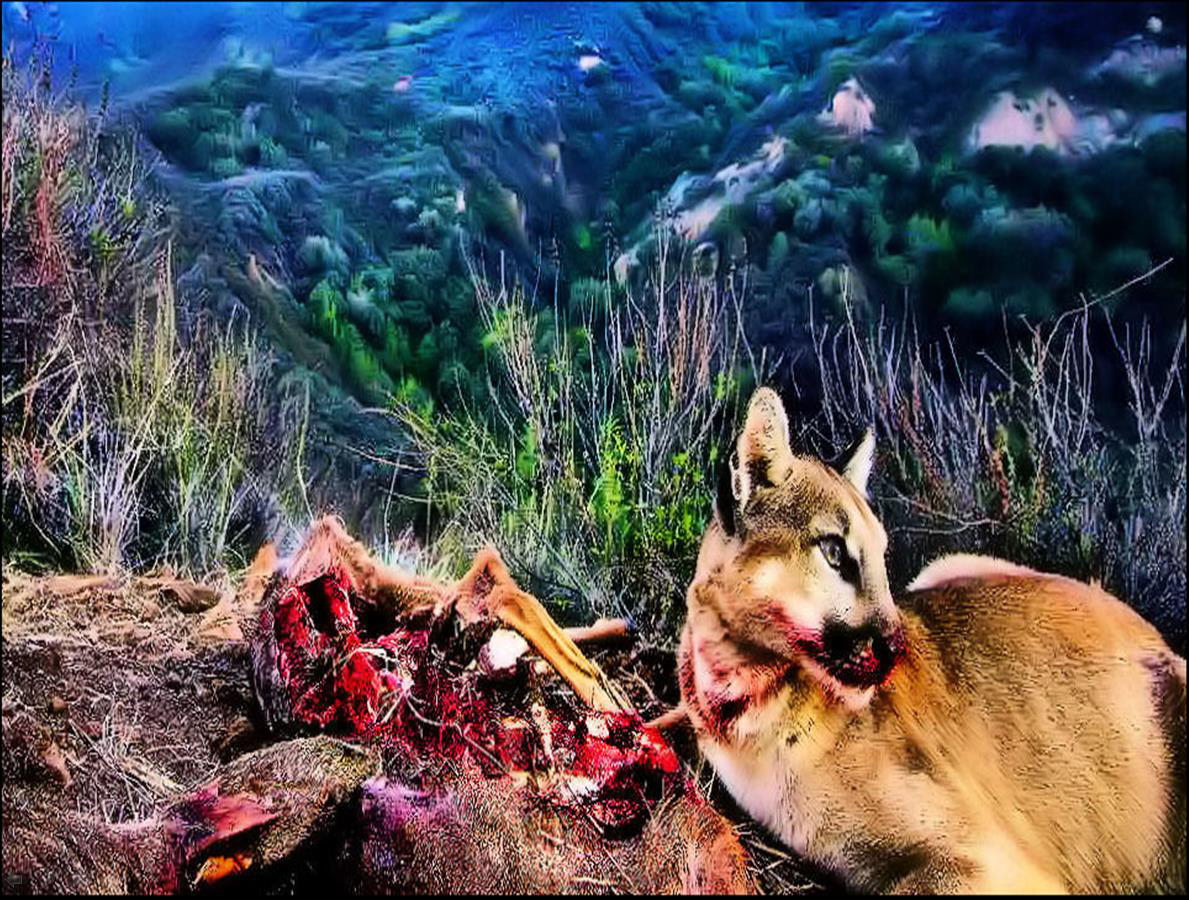
\includegraphics[width=0.8\linewidth]{predator_prey}
\end{figure}
\end{frame}

%------------------------------------------------

\begin{frame}
\frametitle{Everything is a dynamical system}
\textbf{Mechanical system}
\begin{figure}
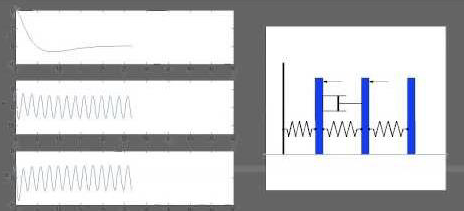
\includegraphics[width=1\linewidth]{mechanical_system}
\end{figure}
\end{frame}

%------------------------------------------------
\section{System theory} 
%------------------------------------------------

\begin{frame}
\frametitle{System theory}
System theory occupies itself with the mathematical description and study of systems.
Models describe the connections between input, output and states.\\
\bigskip
Next to inputs and outputs, states (denoted by \textbf x) are a third type of variable used to describe a system. They represent the internal state of the system at a given time. The next state is a function of the previous states.
The order of a system is the number of state-variables (i.e. the size of the vector \textbf x).\\
\bigskip
Dynamical systems can be devided into two types: \textbf{discrete} and \textbf{continuous} systems.
\end{frame}

%------------------------------------------------
\subsection{Discrete systems} 


\begin{frame}
\frametitle{Discrete systems}

\begin{columns}[c]

\column{.3\textwidth}
\centering \textbf{Delay element}\\
\bigskip
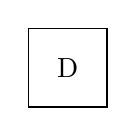
\begin{tikzpicture}
\draw (2,1) rectangle (3,2) node[pos=.5] {D}; 
\end{tikzpicture}

\column{.3\textwidth}
\centering \textbf{Adder}\\
\bigskip
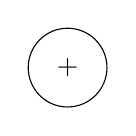
\begin{tikzpicture}
\draw (0,-.8) circle (.5cm) node (0,-.8) {+}; 
\end{tikzpicture}

\column{.3\textwidth}
\centering \textbf{Constant multiplier}\\
\bigskip
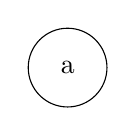
\begin{tikzpicture}
\draw (0,-.8) circle (.5cm) node (0,-.8) {a}; 
\end{tikzpicture}

\end{columns}

\bigskip
Restrictions:
\begin{columns}[c]

\column{.5\textwidth}
\begin{figure}
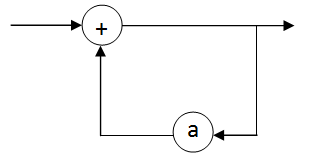
\includegraphics[width=.85\linewidth]{loop}
\end{figure}
No loops without delay element

\column{.5\textwidth}
\begin{figure}
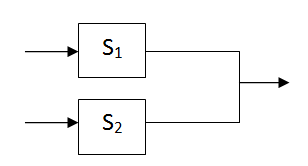
\includegraphics[width=.8\linewidth]{connected_output}
\end{figure}
No connecting outputs without adder

\end{columns}

\end{frame}

%------------------------------------------------

\begin{frame}
\frametitle{Example}
\begin{figure}
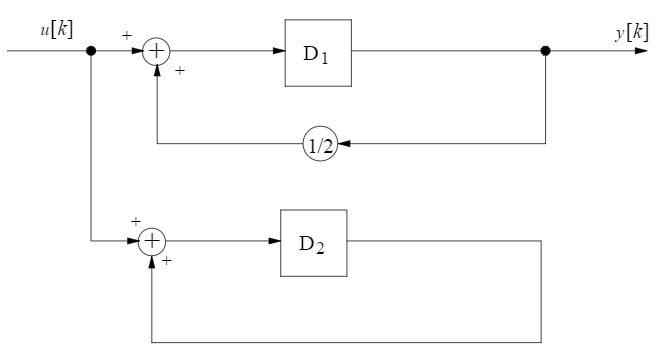
\includegraphics[width=1\linewidth]{discrete_system}
\end{figure}

\end{frame}

%------------------------------------------------

\begin{frame}
\frametitle{Methods}
\textbf{State space representation}\\
$x[k+1] \> = A\; x[k] + B\; u[k]$ \\
$y[k]\qquad = C\; x[k] + C\; u[k]$
\bigskip

\textbf{Difference equations}\\
$\sum\limits_{i=0}^n a_{i}y[k+i] = \sum \limits_{i=0}^n b_{i}u[k+i]$
\bigskip

\textbf{Impulse response}\\
$h[k] = y[k] \> when \> u[k] = \delta[k]$\\
\bigskip

\textbf{Z-transform}\\
$X(z) = \sum \limits_{k = -\infty}^{+\infty} x[k] z^{-k}$
\bigskip

\textbf{Transfer function}\\
$H(z) = \frac{Y(z)}{U(z)} \; \Rightarrow \> Y(z) = H(z)U(z)$

\end{frame}

%------------------------------------------------
\subsection{Continuous systems} 

\begin{frame}
\frametitle{Continuous systems}

\begin{columns}[c]

\column{.3\textwidth}
\centering \textbf{Integrator}\\
\bigskip
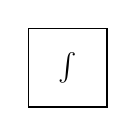
\begin{tikzpicture}
\draw (2,1) rectangle (3,2) node[pos=.5] {$\int$}; 
\end{tikzpicture}

\column{.3\textwidth}
\centering \textbf{Adder}\\
\bigskip
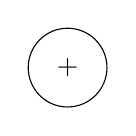
\begin{tikzpicture}
\draw (0,-.8) circle (.5cm) node (0,-.8) {+}; 
\end{tikzpicture}

\column{.3\textwidth}
\centering \textbf{Constant multiplier}\\
\bigskip
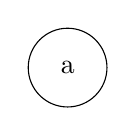
\begin{tikzpicture}
\draw (0,-.8) circle (.5cm) node (0,-.8) {a}; 
\end{tikzpicture}

\end{columns}

\bigskip
Restrictions:
\begin{columns}[c]

\column{.5\textwidth}
\begin{figure}
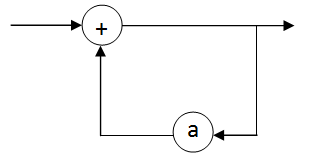
\includegraphics[width=.85\linewidth]{loop}
\end{figure}
No loops without integrator

\column{.5\textwidth}
\begin{figure}
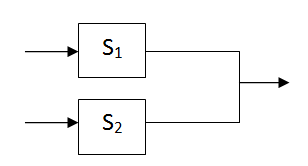
\includegraphics[width=.8\linewidth]{connected_output}
\end{figure}
No connecting outputs without adder

\end{columns}

\end{frame}

%------------------------------------------------

\begin{frame}
\frametitle{Example}
\begin{figure}
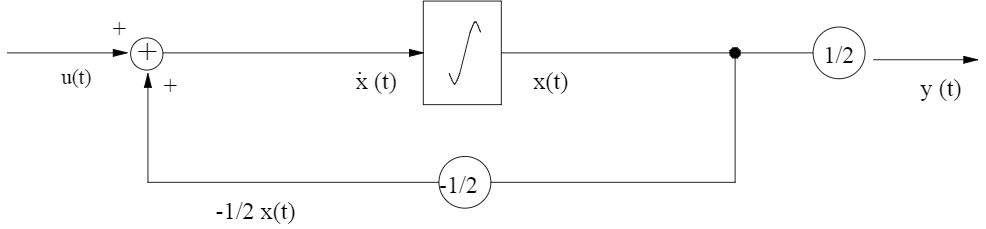
\includegraphics[width=1\linewidth]{continuous_system}
\end{figure}

\end{frame}
%------------------------------------------------

\begin{frame}
\frametitle{Methods}
\textbf{State space representation}\\
$\dot{x}(t) \> = A \;x(t) + B\; u(t)$ \\
$y(t)\> = C\; x(t) + C\; u(t)$
\bigskip

\textbf{Differential equations}\\
$\sum\limits_{i=0}^n a_{i}y^{(i)} = \sum \limits_{i=0}^n b_{i}u^{(i)}$
\bigskip

\textbf{Impulse response}\\
$h(t) = y(t) \> when \> u(t) = \delta(t)$\\
\bigskip

\textbf{Laplace transform}\\
$X(s) = \int_0^\infty \! e^{-st}f(t) \, \mathrm{d}t$
\bigskip

\textbf{Transfer function}\\
$H(s) = \frac{Y(s)}{U(s)} \; \Rightarrow \> Y(s) = H(s)U(s)$

\end{frame}

%------------------------------------------------
\section{Control theory}
%------------------------------------------------

\begin{frame}
\frametitle{Control theory}
Control theory deals with the behavior of dynamical systems and how their behavior is modified by feedback.\\
The output is compared to the desired output and the error is used to adjust the system. 
\bigskip
\begin{figure}
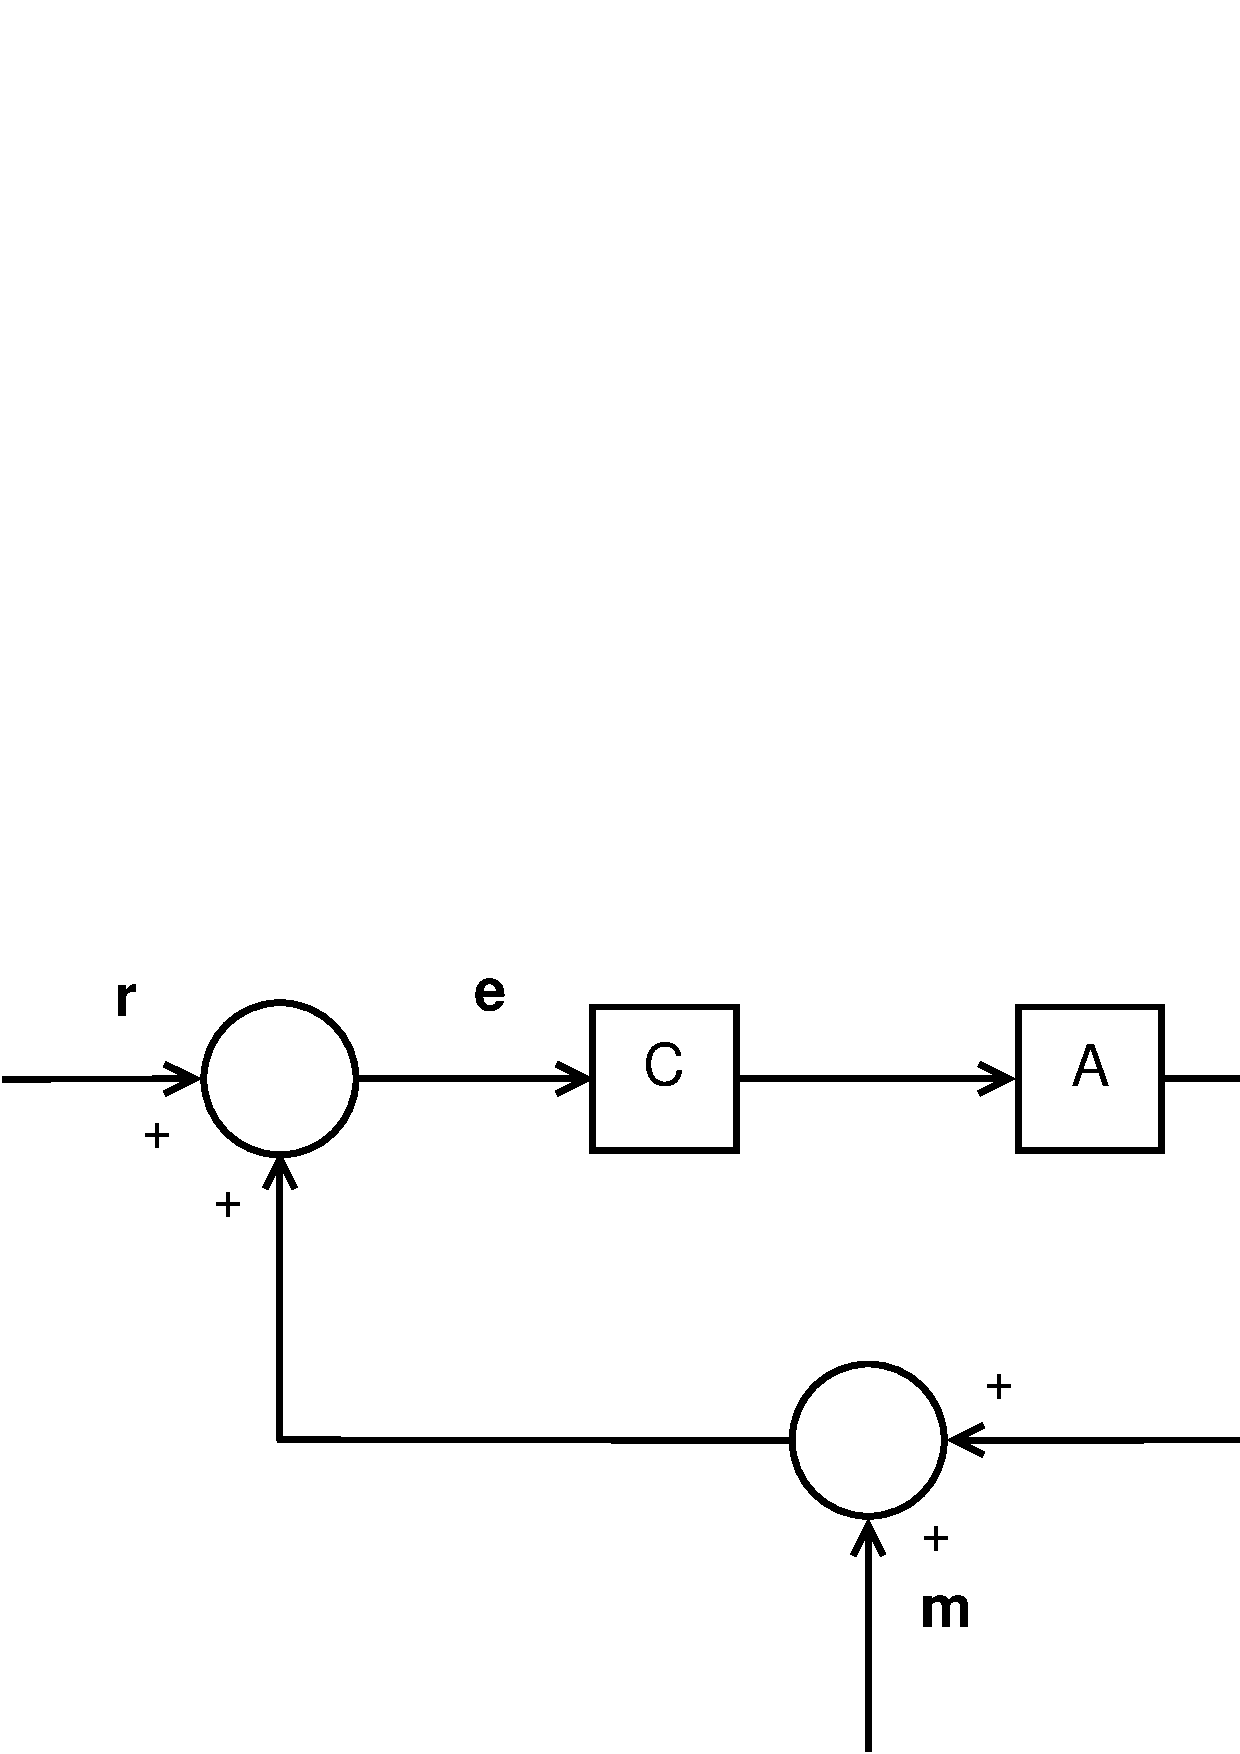
\includegraphics[width=1\linewidth]{full_system1}
\end{figure}
\end{frame}

%------------------------------------------------

\begin{frame}
\vspace{-4ex}
\frametitle{Control theory}
\begin{figure}
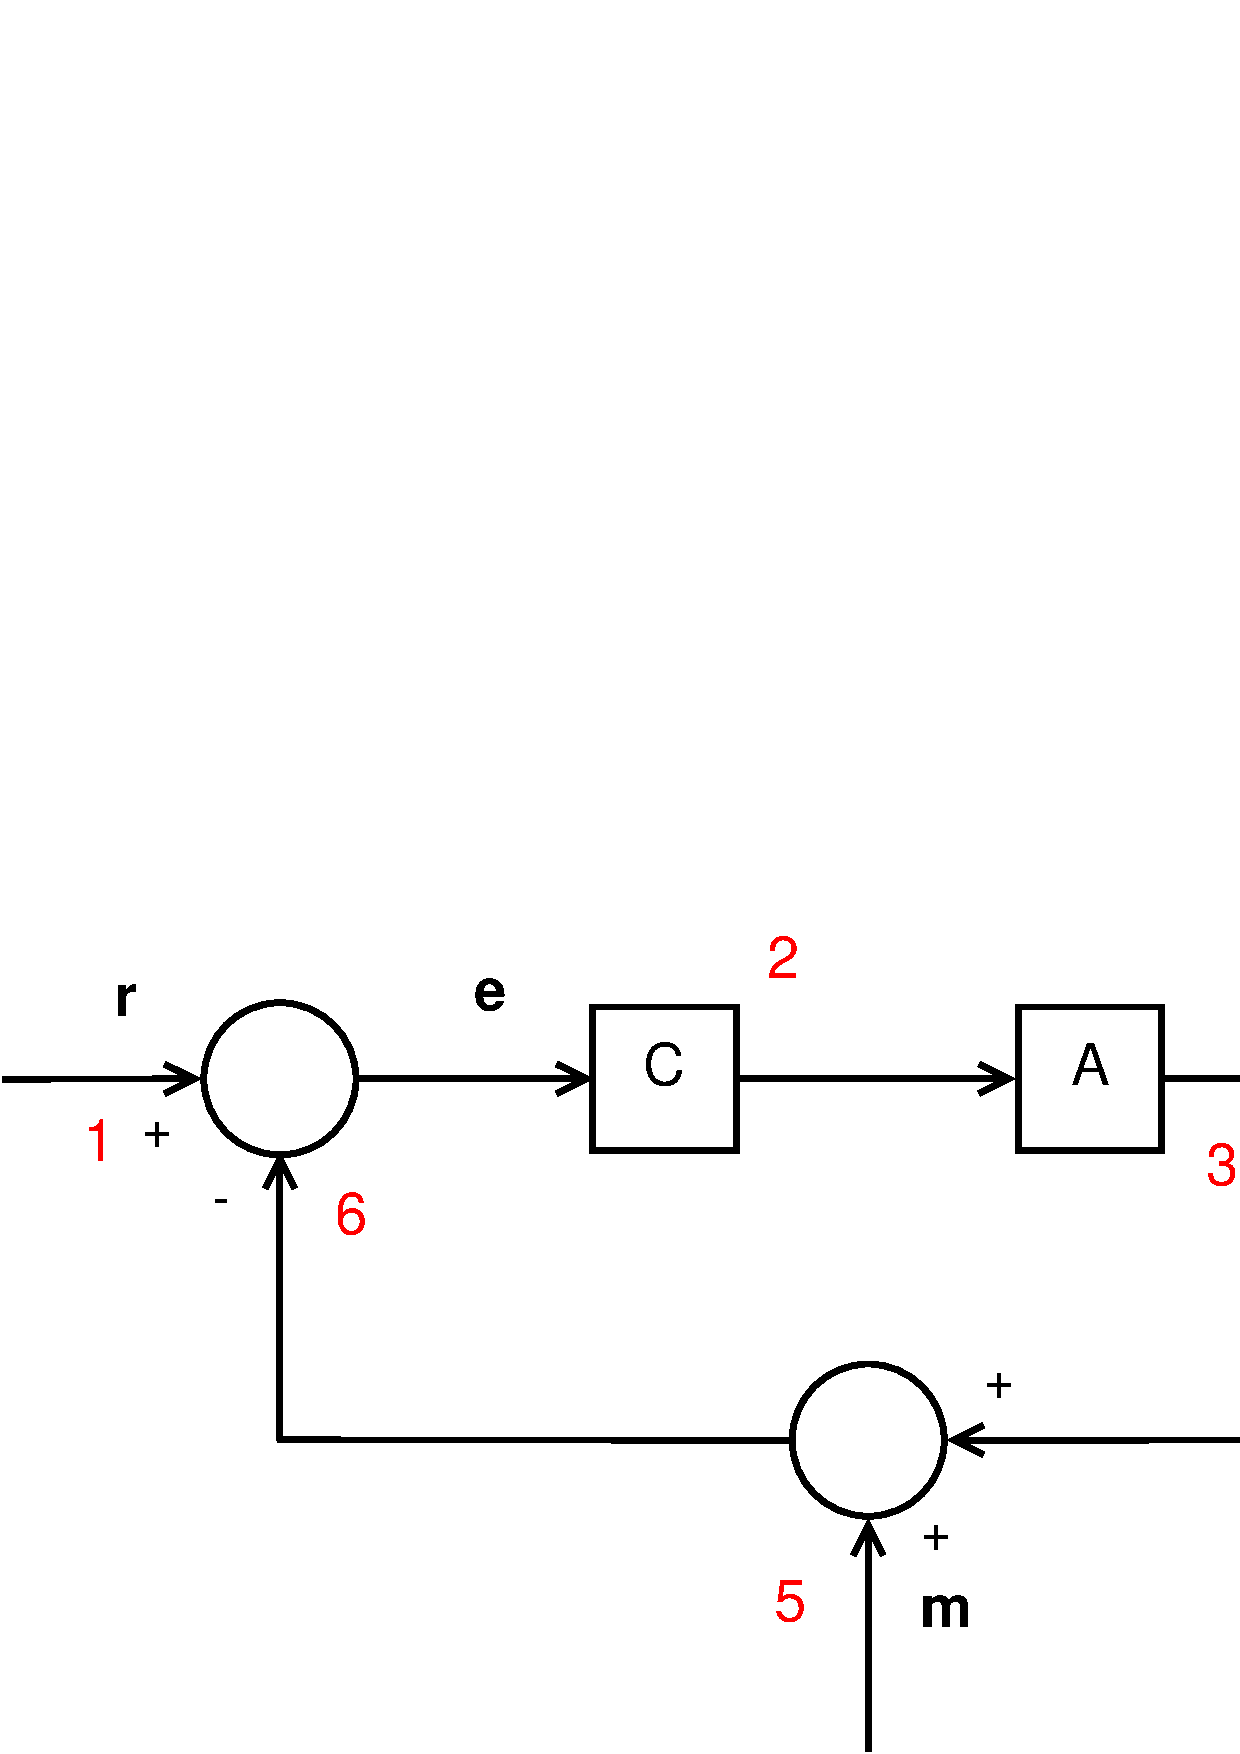
\includegraphics[width=1\linewidth]{full_system2}
\end{figure}
\vspace{-4ex}
1. reference signals: the desired output signals\\
2. controller with model (controller = dynamic)\\
3. actuators that control the system\\
4. Noise\\
5. Measurement noise\\
6. Negative feedback $\rightarrow$ system = stable 
\end{frame}

%------------------------------------------------

\begin{frame}
\frametitle{Open loop}
In an open loop system, the output is not fed back into the controller. Therefore, the controller cannot \textit{'see'} the effect of its actions. \\
This way it is hard to get the desired output.\\
\medskip
\begin{figure}
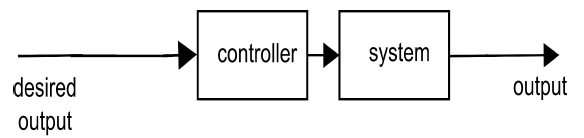
\includegraphics[width=1\linewidth]{open_loop2}
\end{figure}
\bigskip
For example: try pouring water in a glass without looking.
\end{frame}

%------------------------------------------------

\begin{frame}
\frametitle{Feedback}
In a feedback system, the output is fed back to the controller. This way, the  input to the controller becomes the error on the output. 
\medskip
\begin{figure}
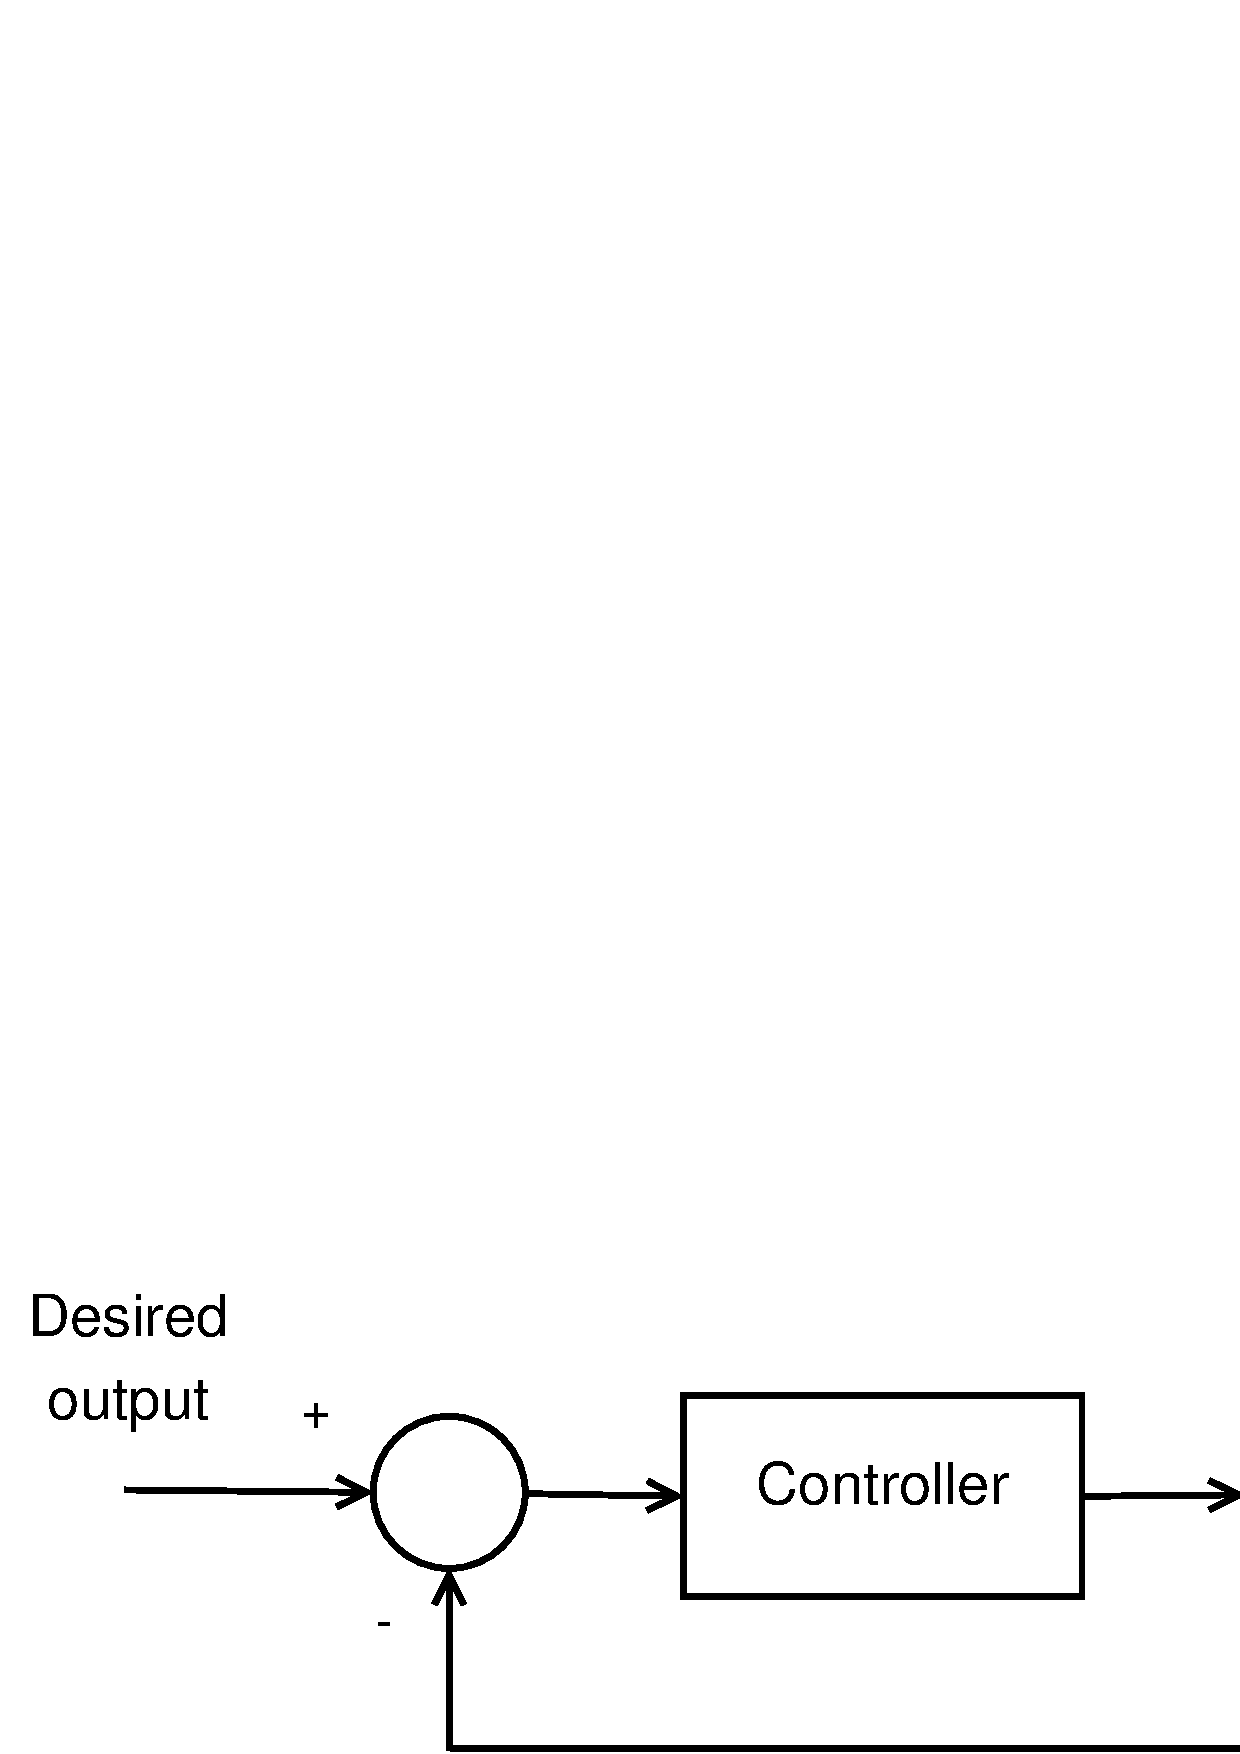
\includegraphics[width=1\linewidth]{closed_loop}
\end{figure}
There are two types of feedback systems. The output can either be added to the desired output (positive feedback) or substracted from it (negative feedback).
\end{frame}

%------------------------------------------------

\begin{frame}
\frametitle{Positive vs. Negative Feedback}
\begin{columns}[c]

\column{.5\textwidth}
\centering \textbf{Negative Feedback}
\begin{enumerate}
\item Continuous behavior
\item Analog technology
\item Output primarily reflects the input
\item Loops enhance of amplify the changes between input and output
\end{enumerate}

\column{.5\textwidth}
\centering \textbf{Positive Feedback}
\begin{enumerate}
\item On-Off behavior
\item Digital Technology
\item Output primarily reflects memory of the past
\item Loops tend to dampen or buffer the changes between input and output
\end{enumerate}

\end{columns}
\end{frame}

%------------------------------------------------

\begin{frame}
\frametitle{Types of controllers}

\vspace{-4ex}
\begin{figure}
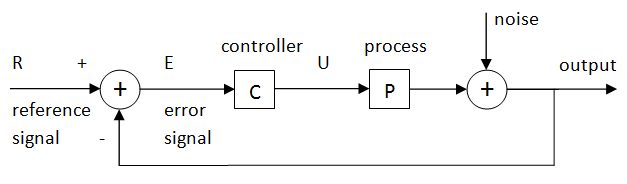
\includegraphics[width=.9\linewidth]{control_theory}
\end{figure}
\vspace{-4ex}
\begin{columns}[c]

\column{.5\textwidth}
\textbf{Proportional controller}\\
$C(s) = K$\\
\medskip
\textbf{Phase lead controller}\\
$C(s) = K \frac{b}{a} \frac{s+a}{s+b} \qquad a<b$\\
\medskip
\textbf{Phase lag controller}\\
$C(s) = K \frac{b}{a} \frac{s+a}{s+b} \qquad a>b$


\column{.5\textwidth}
\center \textbf{PID controller}\\
\begin{figure}
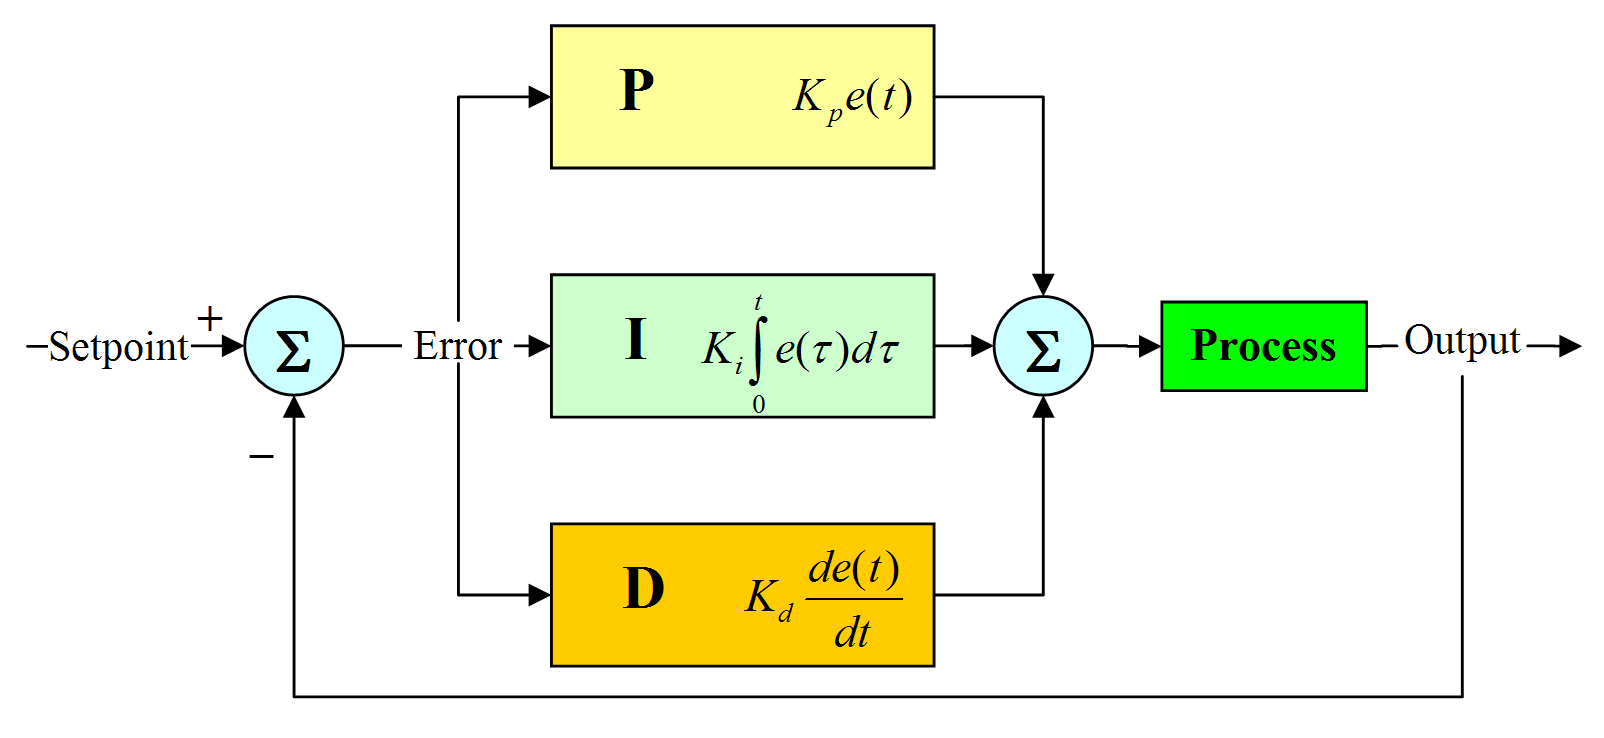
\includegraphics[width=1\linewidth]{PID}
\end{figure}

\end{columns}

\end{frame}

%------------------------------------------------
\section{Examples}
%------------------------------------------------

\begin{frame}
\frametitle{Millenium Bridge London}
Resonance on the Millenium Bridge in London due to the rithm of walking people.
\begin{figure}
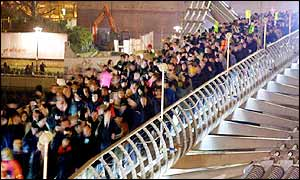
\includegraphics[scale=0.9]{Millenium_bridge}
\end{figure}
\url{https://www.youtube.com/watch?v=eAXVa__XWZ8}
\end{frame}

%------------------------------------------------

\begin{frame}
\frametitle{Feedback in biology}
\begin{figure}
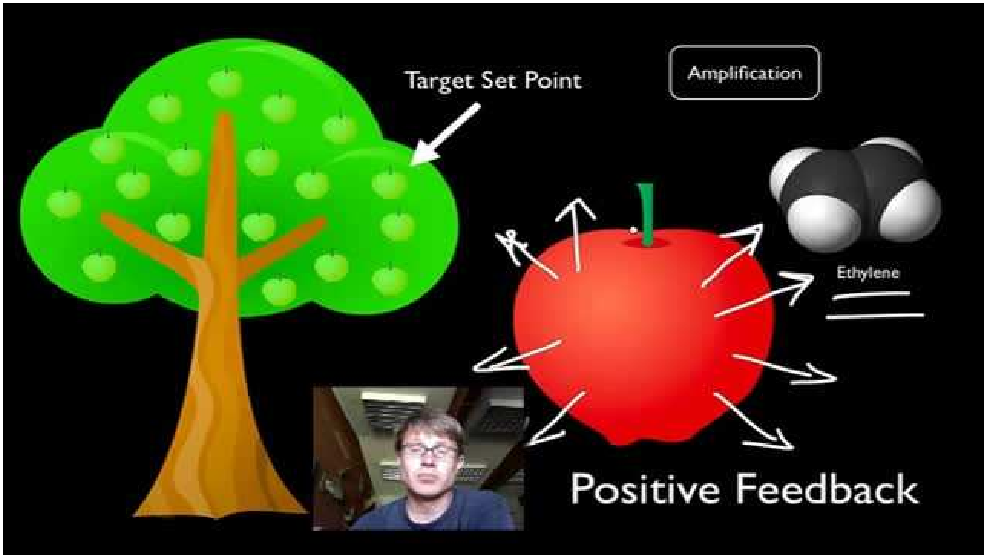
\includegraphics[scale=0.5]{feedback_biology}
\end{figure}
\url{https://youtu.be/CLv3SkF_Eag}
\end{frame}

%------------------------------------------------

\begin{frame}
\frametitle{Autonomous car}
\begin{figure}
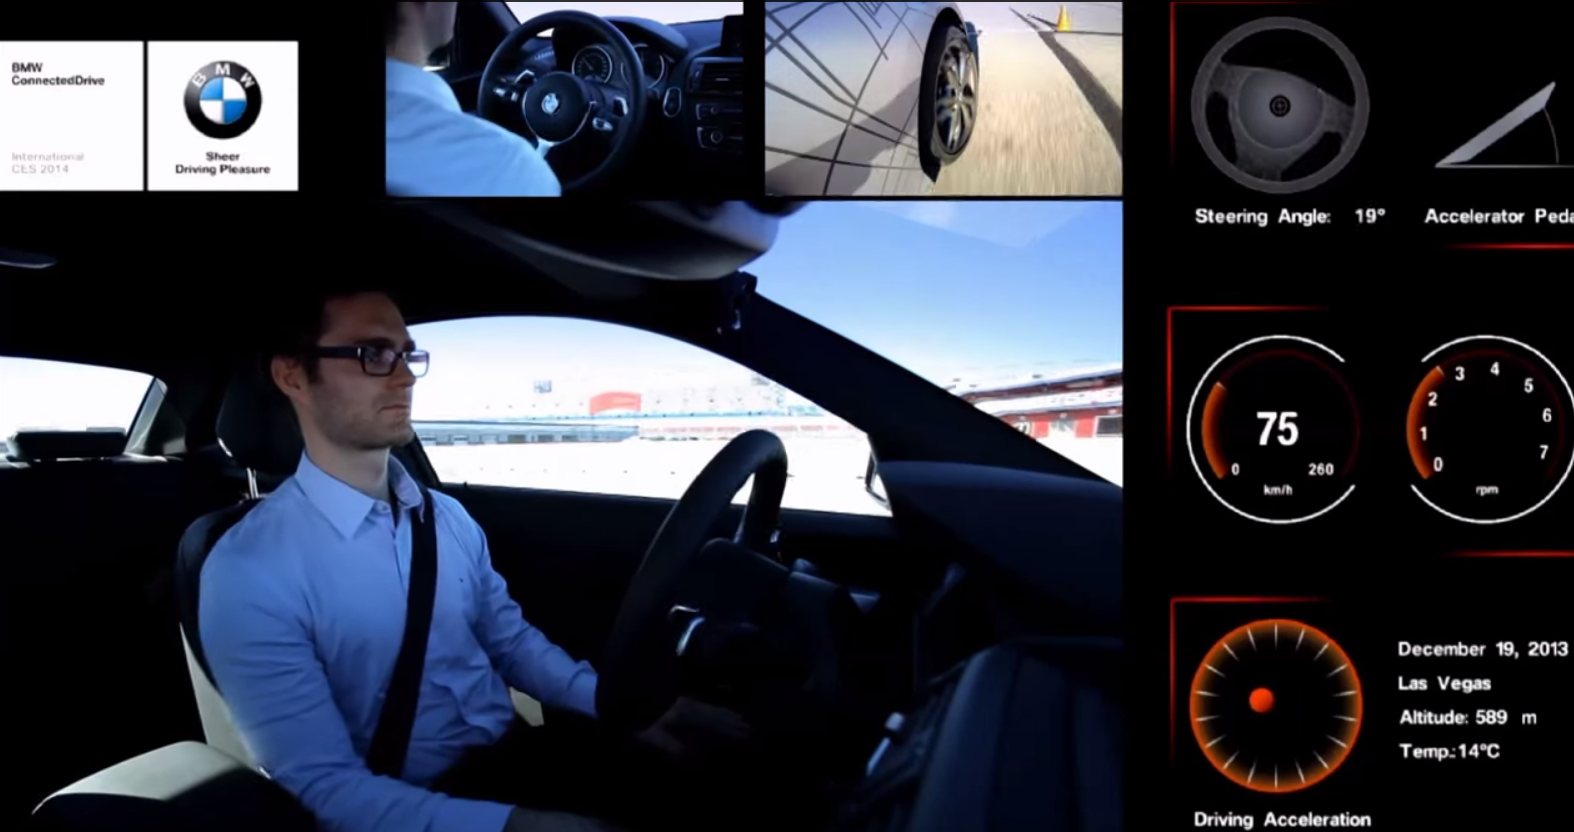
\includegraphics[scale=0.28]{autonomous_car}
\end{figure}
\url{https://youtu.be/1FVglbJZ_tg}
\end{frame}

%------------------------------------------------

\begin{frame}
\frametitle{Badminton robot}
\begin{figure}
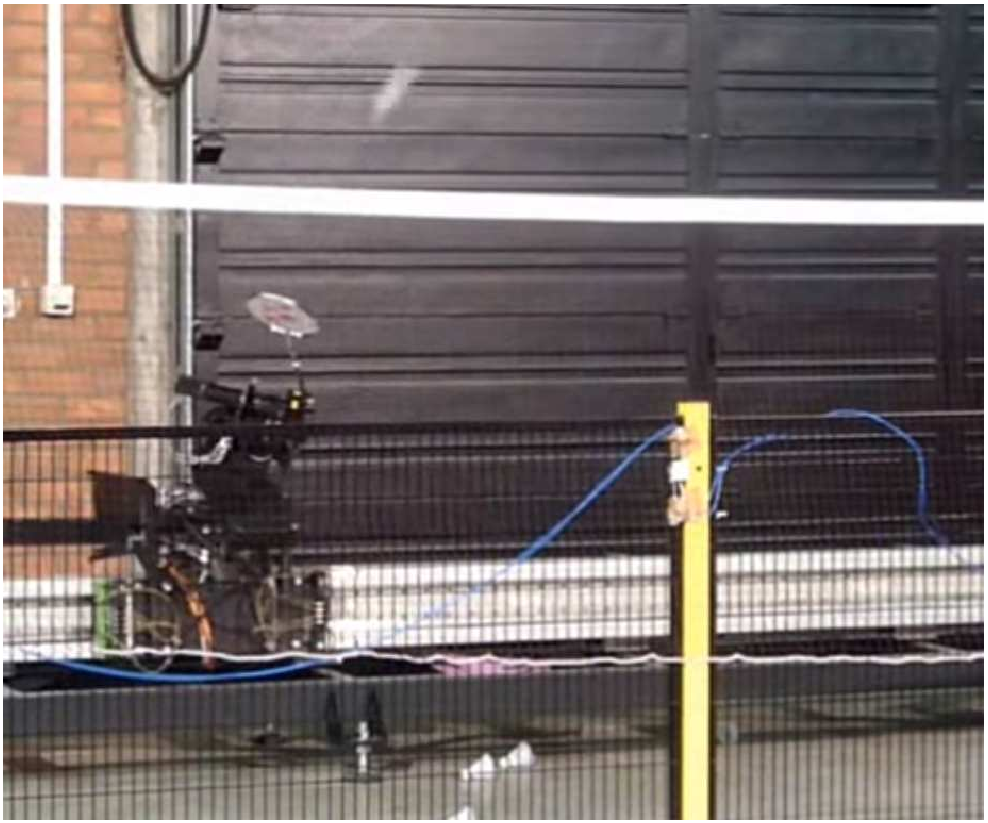
\includegraphics[scale=0.35]{badminton_robot}
\end{figure}
\url{https://youtu.be/LSax71cn6A4}
\end{frame}

%------------------------------------------------

\begin{frame}
\frametitle{Quadcopters}
\begin{figure}
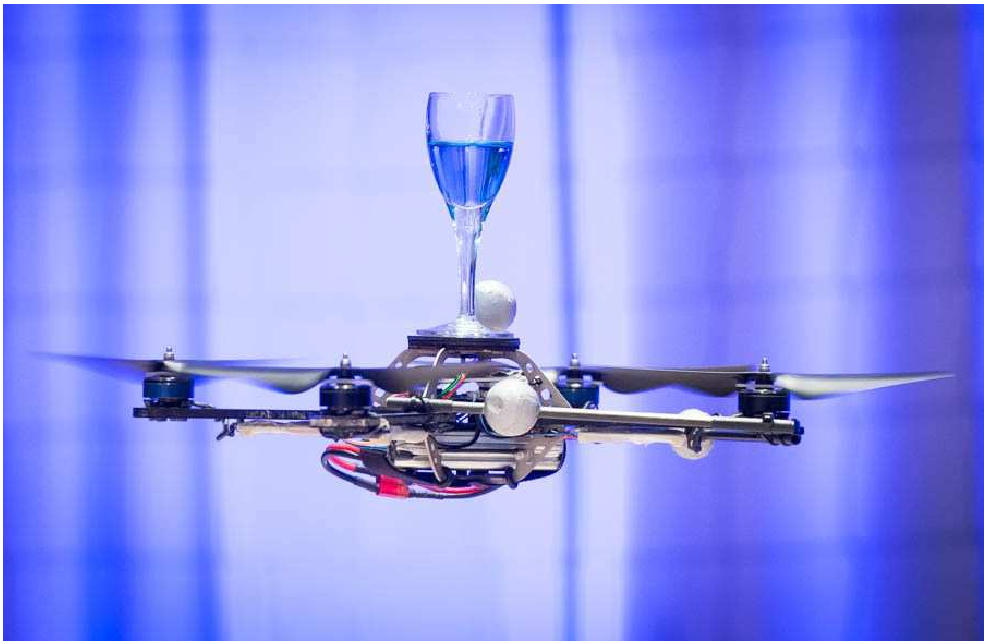
\includegraphics[scale=0.35]{quadcopter}
\end{figure}
\url{https://youtu.be/w2itwFJCgFQ}
\end{frame}

%------------------------------------------------
\end{document} 